\documentclass[letterpaper,12pt]{article}

\usepackage{amsmath,rotating,natbib}
\usepackage[left=1in,right=1in,top=1in,bottom=1in]{geometry}
\bibliographystyle{apsr}

\clubpenalty=10000 \widowpenalty=10000 \hyphenation{matrix}

\begin{document}
\newcommand\var{{\rm Var}}

\title{\textbf{poLCA}: Polytomous Variable\\ Latent Class Analysis \\ \vspace{0.1in} Version 1.4\\}

\author{\\Drew A. Linzer\\
\texttt{dlinzer@emory.edu} \\
Department of Political Science \\
Emory University \\
\\
Jeffrey Lewis \\
\texttt{jblewis@ucla.edu} \\
Department of Political Science \\
University of California, Los Angeles}

\vspace{0.1in}

\date{} \maketitle

\begin{center}
Website: \texttt{https://github.com/dlinzer/poLCA}
\end{center}

\vspace{0.1in}

\begin{abstract}
\noindent \textbf{poLCA} is a software package for the estimation of latent class and latent class regression models for polytomous outcome variables, implemented in the \textsf{R} statistical computing environment. Both models can be called using a single simple command line. The basic latent class model is a finite mixture model in which the component distributions are assumed to be multi-way cross-classification tables with all variables mutually independent. The latent class regression model further enables the researcher to estimate the effects of covariates on predicting latent class membership. \textbf{poLCA} uses expectation-maximization and Newton-Raphson algorithms to find maximum likelihood estimates of the model parameters.
\end{abstract}

\vspace{0.1in}

\newpage

\section{Quick Start}

This section is provided for users who wish to skip the technical details and proceed directly to the estimation of latent class and latent class regression models.

\subsection{Installation}

Download the current version of the \textbf{poLCA} software package from the Comprehensive R Archive Network (CRAN) by opening \textsf{R} and entering
\begin{verbatim}
 > install.packages("poLCA")
\end{verbatim}
Once the installation process is complete, type
\begin{verbatim}
 > library(poLCA)
\end{verbatim}
to load the package into memory.

\subsection{Data and formula definition}

\textbf{poLCA} requires the user to provide a data frame of categorical variables, and a formula definition for the model to be estimated. The data frame may contain missing values (\texttt{NA}), but all other entries must be factors or positive integers.  If the variables are entered as integers, they should contain values that increment from 1 to the maximum number of outcome categories for that variable.

Suppose a data frame \texttt{dat} contains variables \texttt{X1}, \texttt{X2}, \texttt{Y1}, \texttt{Y2}, \texttt{Y3}, and \texttt{Y4}. To estimate a latent class model for the outcome variables \texttt{Y}, define model formula \texttt{f}:
\begin{verbatim}
 > f <- cbind(Y1,Y2,Y3,Y4)~1
\end{verbatim}
To include covariates, modify the formula using the standard \textsf{R} formula expression:
\begin{verbatim}
 > f <- cbind(Y1,Y2,Y3,Y4)~X1+X2
\end{verbatim}
This will estimate the latent class regression model using \texttt{X1} and \texttt{X2} to predict latent class membership.

\subsection{Estimation}

To estimate the latent class model with two latent classes (the default), the command is simply:
\begin{verbatim}
 > lc <- poLCA(f,dat)
\end{verbatim}
Additional classes can be assumed using the \texttt{nclass} argument, as for example:
\begin{verbatim}
 > lc <- poLCA(f,dat,nclass=4)
\end{verbatim}
After estimating the model, \texttt{poLCA} will output selected parameters. Other values of interest are saved as a list in \texttt{lc}.  Further estimation options offered by \texttt{poLCA} are detailed in Section~\ref{s.cmdline}.

\subsection{Global versus local maxima}

It is always advisable to run \texttt{poLCA} more than once to ensure that the global maximum likelihood of the latent class model has been obtained, rather than only a local maximum. This is due to the algorithm that \texttt{poLCA} uses to estimate the parameters of the latent class model. The user may also utilize the \texttt{nrep} argument to automatically re-estimate the model a specified number of times.  For example, the command
\begin{verbatim}
 > lc <- poLCA(f,dat,nclass=4,nrep=10)
\end{verbatim}
will estimate the four-class model ten times and save the one model of the ten that corresponds to the greatest likelihood. For more details, see Section~\ref{s.llmaxima} below.


\section{Motivation for \textbf{poLCA}}

Latent class analysis is a statistical technique for the analysis of multivariate categorical data.  When observed data take the form of a series of categorical responses---as, for example, in public opinion surveys, individual-level voting data, studies of inter-rater reliability, or consumer behavior and decision-making---it is often of interest to investigate sources of confounding between the observed variables, identify and characterize clusters of similar cases, and approximate the distribution of observations across the many variables of interest. Latent class models are a useful tool for accomplishing these goals.

The latent class model seeks to stratify the cross-classification table of observed (or, ``manifest'') variables by an unobserved (``latent'') unordered categorical variable that eliminates all confounding between the manifest variables.  Conditional upon values of this latent variable, responses to all of the manifest variables are assumed to be statistically independent; an assumption typically referred to as ``conditional'' or ``local'' independence.  The model, in effect, probabilistically groups each observation into a ``latent class,'' which in turn produces expectations about how that observation will respond on each manifest variable. Although the model does not automatically determine the number of latent classes in a given data set, it does offer a variety of parsimony and goodness of fit statistics that the researcher may use in order to make a theoretically and empirically sound assessment.

Because the unobserved latent variable is nominal, the latent class model is actually a type of finite mixture model.  The component distributions in the mixture are cross-classification tables of equal dimension to the observed table of manifest variables, and, following the assumption of conditional independence, the frequency in each cell of each component table is simply the product of the respective class-conditional marginal frequencies (the parameters estimated by the latent class model are the proportion of observations in each latent class, and the probabilities of observing each response to each manifest variable, conditional on latent class). A weighted sum of these component tables forms an approximation (or, density estimate) of the distribution of cases across the cells of the observed table. Observations with similar sets of responses on the manifest variables will tend to cluster within the same latent classes.  The model may also be fit to manifest variables that are ordinal, but they will be treated as nominal. In practice, this does not usually restrict analyses in any meaningful way.

An extension of this basic model permits the inclusion of covariates to predict latent class membership.  Whereas in the basic model, every observation has the same probability of belonging to each latent class prior to observing the responses to the manifest variables, in the more general latent class ``regression'' model, these prior probabilities vary by individual as a function of some set of independent (or, ``concomitant'') variables.

\textbf{poLCA} is the first \textsf{R} package to enable the user to estimate latent class models for manifest variables with any number of possible outcomes, and it is the only package that estimates latent class regression models with covariates \citep{poLCA, R}.  The two other \textsf{R} commands that currently exist to estimate latent class models---the \texttt{lca} command in package \textbf{e1071}, and the \texttt{randomLCA} command in package \textbf{randomLCA}---can only accommodate dichotomous outcome variables.

Note that there is occasionally some confusion over the term ``latent class regression'' (LCR); in practice it can have two meanings. In \textbf{poLCA}, LCR models refer to latent class models in which the probability of latent class membership is predicted by one or more covariates.  In other contexts, however, LCR is used to refer to regression models in which the dependent variable is partitioned into latent classes as part of estimating the regression model. It is a way to simultaneously fit more than one regression to the data when the latent data partition is unknown. The \texttt{flexmix} command in package \textbf{flexmix} will estimate this other type of LCR model. Because of these terminology issues, the LCR models estimated using \textbf{poLCA} are sometimes termed ``latent class models with covariates'' or ``concomitant-variable latent class analysis,'' both of which are accurate descriptions of this model.


\section{Latent class models}

The basic latent class model is a finite mixture model in which the component distributions are assumed to be multi-way cross-classification tables with all variables mutually independent. This model was originally proposed by \citet{Lazarsfeld1950} under the name ``latent structure analysis.'' Chapter 13 in \citet{Agresti2002} details the connection between latent class models and finite mixture models.

\subsection{Terminology and model definition}

Suppose we observe $J$ polytomous categorical variables (the ``manifest'' variables), each of which contains $K_j$ possible outcomes, for individuals $i=1...N$. The manifest variables may have different numbers of outcomes, hence the indexing by $j$. Denote as $Y_{ijk}$ the observed values of the $J$ manifest variables such that $Y_{ijk}=1$ if respondent $i$ gives the $k$th response to the $j$th variable, and $Y_{ijk}=0$ otherwise, where $j=1 \ldots J$ and $k=1 \ldots K_j$.

The latent class model approximates the observed joint distribution of the manifest variables as the weighted sum of a finite number, $R$, of constituent cross-classification tables.  $R$ is fixed prior to estimation on the basis of either theoretical reasons or model fit; this issue is addressed in greater detail in Section~\ref{s.model-selection} below.  Let $\pi_{jrk}$ denote the class-conditional probability that an observation in class $r=1 \ldots R$ produces the $k$th outcome on the $j$th variable. Within each class, for each manifest variable, therefore, $\sum_{k=1}^{K_j} \pi_{jrk}=1$.  Further denote as $p_r$ the $R$ mixing proportions that provide the weights in the weighted sum of the component tables, with $\sum_r p_r=1$.

The probability that an individual $i$ in class $r$ produces a particular set of $J$ outcomes on the manifest variables, assuming local independence, is the product
\begin{equation}
f(Y_i;\pi_r) = \prod_{j=1}^J \prod_{k=1}^{K_j}
(\pi_{jrk})^{Y_{ijk}}.\label{eq.probf}
\end{equation}
The probability density function across all classes is the weighted sum
\begin{equation}
\Pr(Y_i | \pi, p) = \sum_{r=1}^R p_r \prod_{j=1}^J \prod_{k=1}^{K_j}
(\pi_{jrk})^{Y_{ijk}}.
\end{equation}
The parameters estimated by the latent class model are $p_r$ and
$\pi_{jrk}$.

Given estimates $\hat p_r$ and $\hat \pi_{jrk}$ of $p_r$ and $\pi_{jrk}$, respectively, the posterior probability that each individual belongs to each class, conditional on the observed values of the manifest variables, can be calculated using Bayes' formula:
\begin{equation}
\widehat{\Pr}(r|Y_i) =\frac{\hat p_r f(Y_i;\hat \pi_r)}{\sum_{q=1}^R \hat p_q f(Y_i;\hat \pi_q)}. \label{eq.posterior}
\end{equation}
Recall that the $\hat \pi_{jrk}$ are estimates of outcome probabilities \emph{conditional on} class $r$.

It is important to remain aware that the number of independent parameters estimated by the latent class model increases rapidly with $R$, $J$, and $K_j$. Given these values, the number of parameters is $R \sum_j (K_j-1) + (R-1)$.  If this number exceeds either the total number of observations, or one fewer than the total number of cells in the cross-classification table of the manifest variables, then the latent class model will be unidentified.

\subsection{Parameter estimation}

\textbf{poLCA} estimates the latent class model by maximizing the log-likelihood function
\begin{equation}
\ln L = \sum_{i=1}^N \ln \sum_{r=1}^R p_r \prod_{j=1}^J
\prod_{k=1}^{K_j} (\pi_{jrk})^{Y_{ijk}} \label{eq.loglik}
\end{equation}
with respect to $p_r$ and $\pi_{jrk}$, using the expectation-maximization (EM) algorithm \citep{DLR1977}.  This log-likelihood function is identical in form to the standard finite mixture model log-likelihood.  As with any finite mixture model, the EM algorithm is applicable because each individual's class membership is unknown and may be treated as missing data \citep{McLachlanKrishnan1997, McLachlanPeel2000}.

The EM algorithm proceeds iteratively. Begin with arbitrary initial values of $\hat{p}_r$ and $\hat \pi_{jrk}$, and label them $\hat{p}_r^{old}$ and $\hat \pi_{jrk}^{old}$. In the expectation step, calculate the ``missing'' class membership probabilities using Eq.~\ref{eq.posterior}, substituting in $\hat{p}_r^{old}$ and $\hat \pi_{jrk}^{old}$.  In the maximization step, update the parameter estimates by maximizing the log-likelihood function given these posterior $\widehat{\Pr}(r|Y_i)$, with
\begin{equation}
\hat{p}_r^{new} = \frac{1}{N} \sum_{i=1}^N \widehat{\Pr}(r|Y_i)
\label{eq.update_p}
\end{equation}
as the new prior probabilities and
\begin{equation}
\hat{\pi}_{jr}^{new} = \frac{\sum_{i=1}^N Y_{ij}
\widehat{\Pr}(r|Y_i)}{\sum_{i=1}^N \widehat{\Pr}(r|Y_i)}
\label{eq.update_pi}
\end{equation}
as the new class-conditional outcome probabilities (see \citet{EverittHand1981, Everitt1984}). In Eq.~\ref{eq.update_pi}, $\hat{\pi}_{jr}^{new}$ is the vector of length $K_j$ of class-$r$ conditional outcome probabilities for the $j$th manifest variable; and $Y_{ij}$ is the $N \times K_j$ matrix of observed outcomes $Y_{ijk}$ on that variable. The algorithm repeats these steps, assigning the new to the old, until the overall log-likelihood reaches a maximum and ceases to increment beyond some arbitrarily small value.

\textbf{poLCA} takes advantage of the iterative nature of the EM algorithm to make it possible to estimate the latent class model even when some of the observations on the manifest variables are missing. Although \textbf{poLCA} does offer the option to listwise delete observations with missing values before estimating the model, it is not necessary to do so. Instead, when determining the product in Eq.~\ref{eq.probf} and the sum in the numerator of Eq.~\ref{eq.update_pi}, \textbf{poLCA} simply excludes from the calculation any manifest variables with missing observations.  The priors are updated in Eq.~\ref{eq.posterior} using as many or as few manifest variables as are observed for each individual.

Depending on the initial values chosen for $\hat{p}_r^{old}$ and $\hat \pi_{jrk}^{old}$, and the complexity of the latent class model being estimated, the EM algorithm may only find a local maximum of the log-likelihood function, rather than the desired global maximum.  For this reason, it is best to re-estimate a particular model a couple of times when using \textbf{poLCA}, in an attempt to find the global maximizer to be taken as the maximum likelihood solution.

\subsection{Standard error estimation} \label{s.lc-se}

\textbf{poLCA} estimates standard errors of the estimated class-conditional response probabilities $\hat \pi_{jrk}$ and the mixing parameters $\hat p_r$ using the \emph{empirical observed} information matrix \citep{Meilijson1989}, which, following \citet[66]{McLachlanPeel2000}, equals
\begin{equation}
\boldsymbol{I_e}(\hat \Psi;Y) = \sum_{i=1}^N \boldsymbol{s}(Y_i;\hat
\Psi)\boldsymbol{s}^T(Y_i;\hat \Psi), \label{eq.I_e}
\end{equation}
where $\boldsymbol{s}(Y_i;\hat \Psi)$ is the score function with respect to the vector of parameters $\Psi$ for the $i$th observation, evaluated at the maximum likelihood estimate $\hat \Psi$;
\begin{equation}
\boldsymbol{s}(Y_i;\Psi) = \sum_{r=1}^R \theta_{ir} \partial \{ \ln
p_r + \sum_{j=1}^J \sum_{k=1}^{K_j} Y_{ijk} \ln \pi_{jrk} \} /
\partial \Psi \label{eq.score}
\end{equation}
where $\theta_{ir}=\widehat{\Pr}(r|Y_i)$ is the posterior probability that observation $i$ belongs to class $r$ (Eq.~\ref{eq.posterior}). The covariance matrix of the parameter estimates is then approximated by the inverse of $\boldsymbol{I_e}(\hat \Psi;Y)$.

Because of the sum-to-one constraint on the $\pi_{jrk}$ across each manifest variable, it is useful to reparameterize the score function in terms of log-ratios $\phi_{jrk} = \ln (\pi_{jrk} / \pi_{jr1})$ for given outcome variable $j$ and class $r$. Then, for the $l$th response on the $h$th item in the $q$th class,
\begin{equation}
\boldsymbol{s}(Y_i;\phi_{hql}) = \theta_{iq} ( Y_{ihl} - \pi_{hql}).
\label{eq.score_phi}
\end{equation}
Likewise, denoting $\omega_r = \ln (p_r/p_1)$, then for the log-ratio corresponding to the $q$th mixing parameter,
\begin{equation}
\boldsymbol{s}(Y_i;\omega_q) = \theta_{iq} - p_{q}.
\label{eq.score_omega}
\end{equation}

To transform the covariance matrix of these log-ratios back to the original units of $\pi$ and $p$, we apply the delta method. For the response probabilities, let $g(\phi_{jrk}) = \pi_{jrk} = e^{\phi_{jrk}} / \sum_l e^{\phi_{jrl}}$. Taking as $\var(\hat \phi)$ the submatrix of the inverse of $\boldsymbol{I_e}(\hat \Psi;Y)$ corresponding to the $\phi$ parameters, then $$ \var(g(\hat \phi)) = g'(\phi) \var(\hat \phi) g'(\phi)^T $$ where $g'(\phi)$ is the Jacobian consisting of elements
\begin{equation*}
\frac{\partial g(\phi_{jrk})}{\partial \phi_{hql}}=
\begin{cases}
0 & \text{ if } q \neq r \\
0 & \text{ if } q=r \text{ but } h \neq j \\
-\pi_{jrk} \pi_{jrl} & \text{ if } q=r \text{ and } h=j \text{ but } l \neq k \\
\pi_{jrk}(1-\pi_{jrk}) & \text{ if } q=r \text{ and } h=j \text{ and
} l=k.
\end{cases}
\end{equation*}
For the mixing parameters, similarly let $h(\omega_r) = p_r = e^{p_r} / \sum_q e^{p_q}$. Taking as $\var(\hat \omega)$ the submatrix of the inverse of $\boldsymbol{I_e}(\hat \Psi;Y)$ corresponding to the $\omega$ parameters, then $$ \var(h(\hat \omega)) = h'(\omega) \var(\hat \omega) h'(\omega)^T $$ where $h'(\omega)$ is the Jacobian consisting of elements
\begin{equation*}
\frac{\partial h(\omega_r)}{\partial \omega_q}=
\begin{cases}
-p_r p_q   & \text{ if } q \neq r \\
p_r(1-p_r) & \text{ if } q=r.
\end{cases}
\end{equation*}
Standard errors of each parameter estimate are equal to the square root of the values along the main diagonal of covariance matrices $\var(\pi)$ and $\var(p)$.


\subsection{Model selection and goodness of fit criteria} \label{s.model-selection}

One of the benefits of latent class analysis, in contrast to other statistical techniques for clustered data, is the variety of tools available for assessing model fit and determining an appropriate number of latent classes $R$ for a given data set.  In some applications, the number of latent classes will be selected for primarily theoretical reasons.  In other cases, however, the analysis may be of a more exploratory nature, with the objective being to locate the best fitting or most parsimonious model.  The researcher may then begin by fitting a complete ``independence'' model with $R=1$, and then iteratively increasing the number of latent classes by one until a suitable fit has been achieved.

Adding an additional class to a latent class model will increase the fit of the model, but at the risk of fitting to noise, and at the expense of estimating a further $1+\sum_j(K_j-1)$ model parameters.  Parsimony criteria seek to strike a balance between over- and under-fitting the model to the data by penalizing the log-likelihood by a function of the number of parameters being estimated. The two most widely used parsimony measures are the Bayesian information criterion, or BIC \citep{Schwartz1978} and Akaike information criterion, or AIC \citep{Akaike1973}. Preferred models are those that minimize values of the BIC and/or AIC. Let $\Lambda$ represent the maximum log-likelihood of the model and $\Phi$ represent the total number of estimated parameters.  Then,
$$ \textrm{AIC} = -2 \Lambda + 2 \Phi $$ and
$$ \textrm{BIC} = -2 \Lambda + \Phi \ln N. $$
\textbf{poLCA} calculates these parameters automatically when estimating the latent class model. The BIC will usually be more appropriate for basic latent class models because of their relative simplicity \citep{LinDayton1997, Forster2000}.

Calculating Pearson's $\chi^2$ goodness of fit and likelihood ratio chi-square ($G^2$) statistics for the observed versus predicted cell counts is another method to determine how well a particular model fits the data \citep{Goodman1970}. Let $q_c$ denote the observed number of cases in each of the $C=\prod K_j$ cells of the cross-classification table of the manifest variables. Let $\hat Q_c$ denote the expected number of cases in each cell under a given model. The $c$th cell (where $c=1 \ldots C$) corresponds to one particular sequence of $J$ outcomes on the manifest variables. Taking the $\hat \pi_{jrk}$ corresponding \emph{only} to those outcomes,
$$ \hat Q_c = N \sum_{r=1}^R \hat p_r \prod_{j=1}^J \hat \pi_{jrk}. $$
The two test statistics are then calculated as
$$ \chi^2 = \sum_c (q_c - \hat Q_c)^2 / \hat Q_c $$ and
$$ G^2 = 2 \sum_c q_c \log (q_c/\hat Q_c). $$

Generally, the goal is to select models that minimize $\chi^2$ or $G^2$ without estimating excessive numbers of parameters.  Note that the distributional assumptions for these statistics are not met if many cells of the observed cross-classification table contain very few observations. Common practice holds that no fewer than 10-20\% of the cells should contain fewer than five observations if either chi-square test is to be used.


\section{Latent class regression models}

The latent class regression model generalizes the basic latent class model by permitting the inclusion of covariates to predict individuals' latent class membership \citep{DaytonMacready1988, HagenaarsMcCutcheon2002}.  This is a so-called ``one-step'' technique for estimating the effects of covariates, because the coefficients on the covariates are estimated simultaneously as part of the latent class model. An alternative estimation procedure that is sometimes used is called the ``three-step'' approach: estimate the basic latent class model, calculate the predicted posterior class membership probabilities using Eq.~\ref{eq.posterior}, and then use these values as the dependent variable(s) in a regression model with the desired covariates. However, as demonstrated by \citet{BCH2004}, the three-step procedure produces biased coefficient estimates.  It is preferable to estimate the entire latent class regression model all at once.

Covariates are included in the latent class regression model through their effects on the priors $p_r$.  In the basic latent class model, it is assumed that every individual has the same prior probabilities of latent class membership. The latent class regression model, in contrast, allows individuals' priors to vary depending upon their observed covariates.

\subsection{Terminology and model definition} \label{s.terminology_r}

Denote the mixing proportions in the latent class regression model as $p_{ri}$ to reflect the fact that these priors are now free to vary by individual. It is still the case that $\sum_r p_{ri}=1$ for each individual. To accommodate this constraint, \textbf{poLCA} employs a generalized (multinomial) logit link function for the effects of the covariates on the priors \citep{Agresti2002}.

Let $X_i$ represent the observed covariates for individual $i$. \textbf{poLCA} arbitrarily selects the first latent class as a ``reference'' class and assumes that the log-odds of the latent class membership priors with respect to that class are linear functions of the covariates. Let $\boldsymbol \beta_r$ denote the vector of coefficients corresponding to the $r$th latent class. With $S$ covariates, the $\boldsymbol \beta_r$ have length $S+1$; this is one coefficient on each of the covariates plus a constant. Because the first class is used as the reference, $\boldsymbol \beta_1=0$ is fixed by definition. Then,
$$ \ln ( p_{2i} / p_{1i} ) = X_i \boldsymbol \beta_2 $$
$$ \ln ( p_{3i} / p_{1i} ) = X_i \boldsymbol \beta_3 $$
$$ \vdots $$
$$ \ln ( p_{Ri} / p_{1i} ) = X_i \boldsymbol \beta_R $$
Following some simple algebra, this produces the general result that
\begin{equation}
p_{ri} = p_r(X_i;\boldsymbol \beta) = \frac{e^{X_i \boldsymbol
\beta_r}}{\sum_{q=1}^R e^{X_i \boldsymbol \beta_q}}.
\label{eq.mlogit}
\end{equation}

The parameters estimated by the latent class regression model are the $R-1$ vectors of coefficients $\boldsymbol \beta_r$ and, as in the basic latent class model, the class-conditional outcome probabilities $\pi_{jrk}$. Given estimates $\boldsymbol{\hat \beta}_r$ and $\hat \pi_{jrk}$ of these parameters, the posterior class membership probabilities in the latent class regression model are obtained by replacing the $p_r$ in Eq.~\ref{eq.posterior} with the function $p_r(X_i;\boldsymbol \beta)$ in Eq.~\ref{eq.mlogit}:
\begin{equation}
\widehat{\Pr}(r|X_i; Y_i) =\frac{p_r(X_i;\boldsymbol{\hat \beta})
f(Y_i;\hat \pi_r)}{\sum_{q=1}^R p_q(X_i;\boldsymbol{\hat \beta})
f(Y_i;\hat \pi_q)}. \label{eq.posterior_r}
\end{equation}
The number of parameters estimated by the latent class regression model is equal to $R \sum_j (K_j-1) + (S+1)(R-1)$. The same considerations mentioned earlier regarding model identifiability also apply here.

\subsection{Parameter estimation}

The latent class regression model log-likelihood function is identical to Eq.~\ref{eq.loglik} except that the function $p_r(X_i;\boldsymbol \beta)$ (Eq.~\ref{eq.mlogit}) takes the place
of $p_r$:
\begin{equation}
\ln L = \sum_{i=1}^N \ln \sum_{r=1}^R p_r(X_i;\boldsymbol \beta)
\prod_{j=1}^J \prod_{k=1}^{K_j} (\pi_{jrk})^{Y_{ijk}}.
\label{eq.loglik_r}
\end{equation}

To find the values of $\boldsymbol{\hat \beta}_r$ and $\hat \pi_{jrk}$ that maximize this function, \textbf{poLCA} uses a modified EM algorithm with a Newton-Raphson step, as set forth by \citet{BRMZR1997}. This estimation process begins with initial values of $\boldsymbol{\hat \beta}_r^{old}$ and $\hat \pi_{jrk}^{old}$ that are used to calculate posterior probabilities $\widehat{\Pr}(r|X_i; Y_i)$ (Eq.~\ref{eq.posterior_r}).  The coefficients on the concomitant variables are updated according to the formula
\begin{equation}
\boldsymbol{\hat \beta}_r^{new} = \boldsymbol{\hat \beta}_r^{old} +
(- \mathbf D_{\boldsymbol \beta}^2 \log L)^{-1} \mathbf
D_{\boldsymbol \beta} \log L
\end{equation}
where \textbf{D}$_{\boldsymbol \beta}$ is the gradient and \textbf{D}$_{\boldsymbol \beta}^2$ the Hessian matrix with respect to $\boldsymbol \beta$. The $\hat \pi_{jrk}^{new}$ are updated as
\begin{equation}
\hat{\pi}_{jr}^{new} = \frac{\sum_{i=1}^N Y_{ij}
\widehat{\Pr}(r|X_i; Y_i)}{\sum_{i=1}^N \widehat{\Pr}(r|X_i; Y_i)}.
\end{equation}
These steps are repeated until convergence, assigning the new parameter estimates to the old in each iteration.  The formulas for the gradient and Hessian matrix are provided in \citet{BRMZR1997}.

Because all of the concomitant variables must be observed in order to calculate $p_{ri}$ (Eq.~\ref{eq.mlogit}), \textbf{poLCA} listwise deletes cases with missing values on the $X_i$ before estimating the latent class regression model. However, missing values on the manifest variables $Y_i$ can be accommodated in the latent class regression model, just as they were in the basic latent class model.

Note that when employing this estimation algorithm, different initial parameter values may lead to different local maxima of the log-likelihood function.  To be more certain that the global maximum likelihood solution has been found, the \texttt{poLCA} function call should always be repeated a handful of times.

\subsection{Standard error estimation}

For latent class models with covariates, standard errors are obtained just as for models without covariates: using the empirical observed information matrix (Eq.~\ref{eq.I_e}).  First, we generalize the score function (Eq.~\ref{eq.score}) so that
\begin{equation}
\boldsymbol{s}(X_i,Y_i;\Psi) = \sum_{r=1}^R \theta_{ir} \partial \{
\ln p_{r}(X_i;\boldsymbol{\beta}) + \sum_{j=1}^J \sum_{k=1}^{K_j}
Y_{ijk} \ln \pi_{jrk} \} / \partial \Psi.
\end{equation}
As before, $\theta_{ir}$ denote posterior probabilities.  Since this function is no different than Eq.~\ref{eq.score} in terms of the $\pi$ parameters, the score function $\boldsymbol{s}(X_i,Y_i;\phi_{hql}) = \boldsymbol{s}(Y_i;\phi_{hql})$ (Eq.~\ref{eq.score_phi}), and the covariance matrix $\var(\pi)$ may be calculated in precisely the same way as for models without covariates.

Now, however, the priors $p_{ri}$ are free to vary by individual as a function of some set of coefficients $\boldsymbol{\beta}$, as given in Eq.~\ref{eq.mlogit}. Letting $q$ index classes and $s$ index covariates,
\begin{equation}
s(X_i,Y_i;\beta_{qs}) = X_{is} (\theta_{iq} - p_{iq}).
\label{eq.score_beta}
\end{equation}
The standard errors of the coefficients $\beta$ are equal to the square root of the values along the main diagonal of the submatrix of the inverse of the empirical observed information matrix corresponding to the $\beta$ parameters. (Note that when the model has no covariates, $X_i=1$ and $p_{iq}=p_q$ (that is, the priors do not vary by individual), so Eq.~\ref{eq.score_beta} reduces to Eq.~\ref{eq.score_omega} as expected.)

To obtain the covariance matrix of the mixing parameters $p_r$, which are the average value across all observations of the priors $p_{ir}$, we apply the delta method.  Let
\begin{equation*}
h(\beta_r) = p_r = \frac{1}{N} \sum_i \left( \frac{e^{X_i
\boldsymbol{\beta_r}}}{\sum_{q=1}^R e^{X_i \boldsymbol{\beta_q}}}
\right).
\end{equation*}
Then $$ \var(h(\hat \beta)) = h'(\beta) \var(\hat \beta) h'(\beta)^T $$ where $h'(\beta)$ is a Jacobian with elements
\begin{equation*}
\frac{\partial h (\beta_r)}{\partial \beta_{qs}}=
\begin{cases}
\frac{1}{N} \sum_i X_{is} (-p_{ir} p_{iq}) & \text{ if } q \neq r \\
\frac{1}{N} \sum_i X_{is} ( p_{ir} (1-p_{ir}) ) & \text{ if } q=r ,
\end{cases}
\end{equation*}
leading directly to the standard errors of interest.


\section{Using \textbf{poLCA}}

The \textbf{poLCA} package makes it possible to estimate a wide range of latent class models in \textsf{R} using a single command line, \texttt{poLCA}. Also included in the package is the command \texttt{poLCA.simdata}, which enables the user to create simulated data sets that match the data-generating process assumed by either the basic latent class model or the latent class regression model. This functionality is useful for testing the \textbf{poLCA} estimator and for performing Monte Carlo-style analyses of latent class models.

Begin by loading the \textbf{poLCA} package into memory in \textsf{R} by entering
\begin{verbatim}
 > library(poLCA)
\end{verbatim}
The internal documentation for the \texttt{poLCA} command may be viewed at any time by entering
\begin{verbatim}
 > ?poLCA
\end{verbatim}

\subsection{Data input and sample data sets}

Data are input to the \texttt{poLCA} function as a data frame containing all manifest and concomitant variables (if needed). \emph{The manifest variables must be coded either as factors, or as integer values starting at one for the first outcome category, and increasing to the maximum number of outcomes for each variable.}  If any of the manifest variables contain zeros, negative values, or decimals, \texttt{poLCA} will produce an error message and terminate without estimating the model. The input data frame may contain missing values.

\textbf{poLCA} also comes pre-installed with five sample data sets that are useful for exploring different aspects of latent class and latent class regression models.
\begin{description}
    \item [\texttt{carcinoma}:] Dichotomous ratings by seven pathologists of 118 slides for the presence or absence of carcinoma in the uterine cervix. Source: \citet[542]{Agresti2002}.
    \item [\texttt{cheating}:] Dichotomous responses by 319 undergraduates to questions about cheating behavior. Also each student's GPA, which is useful as a concomitant variable.  Source: \citet[33 and 85]{Dayton1998}.
    \item [\texttt{election}:] Two sets of six questions with four responses each, asking respondents' opinions of how well various traits describe presidential candidates Al Gore and George~W. Bush. Also potential covariates vote choice, age, education, gender, and party ID. Source: \citet{NES2000}.
    \item [\texttt{gss82}:] Attitudes towards survey taking across two dichotomous and two trichotomous items among 1202 white respondents to the 1982 General Social Survey. Source: \citet[30]{McCutcheon1987}.
    \item [\texttt{values}:] Dichotomous measures of 216 survey respondents' tendencies towards ``universalistic'' or ``particularistic'' values on four questions. Source: \citet{Goodman1974}.
\end{description}
These data sets may be accessed using the \texttt{data(\emph{name})} command.  Examples of models and analyses using the sample data sets are included in the internal documentation for each.

\subsection{\textbf{poLCA} command line options} \label{s.cmdline}

To specify a latent class model, \textbf{poLCA} uses the standard, symbolic \textsf{R} model formula expression. The response variables are the manifest variables of the model.  Because latent class models have multiple manifest variables, these variables must be ``bound'' as \texttt{cbind(Y1,Y2,Y3,...)} in the model formula. For the basic latent class model with no covariates, the formula definition takes the form
\begin{verbatim}
 > f <- cbind(Y1,Y2,Y3)~1
\end{verbatim}
The \verb"~1" instructs \texttt{poLCA} to estimate the basic latent class model. For the latent class regression model, replace the \verb"~1" with the desired function of covariates, as, for example:
\begin{verbatim}
 > f <- cbind(Y1,Y2,Y3)~X1+X2*X3
\end{verbatim}
Further assistance on formula specification in \textsf{R} can be obtained by entering \verb"?formula" at the command prompt.

To estimate the specified latent class model, the default \texttt{poLCA} command is:
\begin{verbatim}
 > poLCA(formula, data, nclass=2, maxiter=1000, graphs=FALSE, tol=1e-10,
         na.rm=TRUE, probs.start=NULL, nrep=1, verbose=TRUE, calc.se=TRUE)
\end{verbatim}
At minimum, it is necessary to enter a formula (as just described) and a data frame (as described in the previous subsection). The remaining options are:
\begin{description}
    \item [\texttt{nclass}:] The number of latent classes to assume in the model; $R$ in the above notation. Setting \texttt{nclass=1} results in \texttt{poLCA} estimating the loglinear independence model \citep{Goodman1970}. The default is two.
    \item [\texttt{maxiter}:] The maximum number of iterations through which the estimation algorithm will cycle.  If convergence is not achieved before reaching this number of iterations, \texttt{poLCA} terminates and reports an error message.  The default is 1000, but this will be insufficient for certain models.
    \item [\texttt{graphs}:] Logical, for whether \texttt{poLCA} should graphically display the parameter estimates at the completion of the estimation algorithm. The default is \texttt{FALSE}.
    \item [\texttt{tol}:] A tolerance value for judging when convergence has been reached.  When the one-iteration change in the estimated log-likelihood is less than \texttt{tol}, the estimation algorithm stops updating and considers the maximum log-likelihood to have been found. The default is $1 \times 10^{-10}$ which is a standard value; this option will rarely need to be invoked.
    \item [\texttt{na.rm}:] Logical, for how \texttt{poLCA} handles cases with missing values on the manifest variables.  If \texttt{TRUE}, those cases are removed (listwise deleted) before estimating the model. If \texttt{FALSE}, cases with missing values are retained.  (As discussed above, cases with missing covariates are always removed.) The default is \texttt{TRUE}.
    \item [\texttt{probs.start}:] A list of matrices of class-conditional response probabilities, $\pi_{jrk}$, to be used as the starting values for the EM estimation algorithm.  Each matrix in the list corresponds to one manifest variable, with one row for each latent class, and one column for each possible outcome.  The default is \texttt{NULL}, meaning that starting values are generated randomly.  Note that if \texttt{nrep} $>1$, then any user-specified \texttt{probs.start} values are only used in the first of the \texttt{nrep} attempts.
    \item [\texttt{nrep}:] Number of times to estimate the model, using different values of \texttt{probs.start}.  The default is one.  Setting \texttt{nrep} $>1$ automates the search for the global---rather than just a local---maximum of the log-likelihood function. \texttt{poLCA} returns only the parameter estimates corresponding to the model producing the greatest log-likelihood.
    \item [\texttt{verbose}:] Logical, indicating whether \texttt{poLCA} should output to the screen the results of the model.  If \texttt{FALSE}, no output is produced. The default is \texttt{TRUE}.
    \item [\texttt{calc.se}:] Logical, indicating whether \texttt{poLCA} should calculate the standard errors of the estimated class-conditional response probabilities and mixing proportions.  The default is \texttt{TRUE}; can only be set to \texttt{FALSE} if estimating a basic model with no concomitant variables specified in \texttt{formula}.
\end{description}

\subsection{\textbf{poLCA} output}

The \texttt{poLCA} function returns an object of class poLCA; a list containing the following elements.
\begin{description}
    \item [\texttt{y}:] A data frame of the manifest variables.
    \item [\texttt{x}:] A data frame of the covariates, if specified.
    \item [\texttt{N}:] Number of cases used in the model.
    \item [\texttt{Nobs}:] Number of fully observed cases (less than or equal to \texttt{N}).
    \item [\texttt{probs}:] A list of matrices containing the estimated class-conditional outcome probabilities $\hat \pi_{jrk}$. Each item in the list represents one manifest variable; columns correspond to possible outcomes on each variable, and rows correspond to the latent classes.
    \item [\texttt{probs.se}:] Standard errors of the estimated class-conditional response probabilities, in the same format as \texttt{probs}.
    \item [\texttt{P}:] The respective size of each latent class; equal to the estimated mixing proportions $\hat p_r$ in the basic latent class model, or the mean of the priors in the latent class regression model.
    \item [\texttt{P.se}:] The standard errors of \texttt{P}.
    \item [\texttt{posterior}:] An $N \times R$ matrix containing each observation's posterior class membership probabilities. Also see the function \texttt{poLCA.posterior}.
    \item [\texttt{predclass}:] A vector of length $N$ of predicted class memberships, by modal assignment.
    \item [\texttt{predcell}:] A table of observed versus predicted cell counts for cases with no missing values.  Also see functions \texttt{poLCA.table} and \texttt{poLCA.predcell}.
    \item [\texttt{llik}:] The maximum value of the estimated model log-likelihood.
    \item [\texttt{numiter}:] The number of iterations required by the estimation algorithm to achieve convergence.
    \item [\texttt{maxiter}:] The maximum number of iterations through which the estimation algorithm was set to run.
    \item [\texttt{coeff}:] An $(S+1) \times (R-1)$ matrix of estimated multinomial logit coefficients $\boldsymbol{\hat \beta}_r$, for the latent class regression model.  Rows correspond to concomitant variables $X$. Columns correspond to the second through $R$th latent classes; see Eq.~\ref{eq.mlogit}.
    \item [\texttt{coeff.se}:] Standard errors of the coefficient estimates, in the same format as \texttt{coeff}.
    \item [\texttt{coeff.V}:] Covariance matrix of the coefficient estimates.
    \item [\texttt{aic}:] Akaike Information Criterion.
    \item [\texttt{bic}:] Bayesian Information Criterion.
    \item [\texttt{Gsq}:] Likelihood ratio/deviance statistic.
    \item [\texttt{Chisq}:] Pearson Chi-square goodness of fit statistic.
    \item [\texttt{time}:] Length of time it took to estimate the model.
    \item [\texttt{npar}:] The number of degrees of freedom used by the model (that is, the number of estimated parameters).
    \item [\texttt{resid.df}:] The number of residual degrees of freedom, equal to the lesser of $N$ and $(\prod_j K_j)-1$, minus \texttt{npar}.
    \item [\texttt{attempts}:] A vector containing the maximum log-likelihood values found in each of the \texttt{nrep} attempts to fit the model.
    \item [\texttt{eflag}:] Logical, error flag. \texttt{TRUE} if estimation algorithm needed to automatically restart with new initial parameters, otherwise \texttt{FALSE}.  A restart is caused in the event of computational/rounding errors that result in nonsensical parameter estimates. If an error occurs, \texttt{poLCA} outputs an error message to alert the user.
    \item [\texttt{probs.start}:] A list of matrices containing the class-conditional response probabilities used as starting values in the EM estimation algorithm.  If the algorithm needed to restart (see \texttt{eflag}), this contains the starting values used for the final, successful, run of the estimation algorithm.
    \item [\texttt{probs.start.ok}:] Logical. \texttt{FALSE} if \texttt{probs.start} was incorrectly specified by the user, otherwise \texttt{TRUE}.
    \item [\texttt{call}:] The \texttt{poLCA} function call entered by the user.
\end{description}
If \texttt{verbose=TRUE}, selected items from this list are displayed automatically once the latent class model has been estimated.

\subsection{Predicted cell frequencies from the latent class model} \label{s.predtable}

The poLCA object contains an element \texttt{predcell} which enables quick comparisons of the observed cell counts to the cell counts predicted by the latent class model---but only for cells that were observed to contain at least one observation.  To generate predicted cell counts for \emph{any} combination of the manifest variables, including cells with zero observations, apply the \texttt{poLCA.table} function to the fitted latent class model stored in the poLCA object.  This function post-processes the latent class model estimates to produce frequency distributions and two-way tables of predicted cell counts, holding the values of the other manifest variables fixed at a user-specified set of values.

As an example, consider a basic two-class latent class model fitted to the four survey variables in the \texttt{gss82} data set included in the \textbf{poLCA} package.
\begin{verbatim}
 > data(gss82)
 > f <- cbind(PURPOSE,ACCURACY,UNDERSTA,COOPERAT)~1
 > gss.lc2 <- poLCA(f,gss82,nclass=2)
\end{verbatim}
Entering \texttt{gss.lc2\$predcell} shows that of the 36 possible four-response sequences of responses ($3 \times 2 \times 2 \times 3$), only 33 are actually observed.  One unobserved sequence is the combination \texttt{PURPOSE}=3, \texttt{ACCURACY}=1, \texttt{UNDERSTA}=2, \texttt{COOPERAT}=3.  We produce the predicted frequency table for \texttt{COOPERAT} conditional on the specified values of the other three variables using the command
\begin{verbatim}
 > poLCA.table(formula=COOPERAT~1,
               condition=list(PURPOSE=3,ACCURACY=1,UNDERSTA=2),
               lc=gss.lc2)
\end{verbatim}
Fitted values of 4.94 for \texttt{COOPERAT}=1 and 0.76 for \texttt{COOPERAT}=2 also appeared in the outputted \texttt{gss.lc2\$predcell}; we may now also see that the fitted value for \texttt{COOPERAT}=3 is 0.16, close to the observed value of zero.

To make a two-way table, modify the specification of the \texttt{formula} argument to contain both a row (\texttt{COOPERAT}) and a column (\texttt{UNDERSTA}) variable, again using the \texttt{condition} argument to hold fixed the values of the other two variables:
\begin{verbatim}
 > poLCA.table(formula=COOPERAT~UNDERSTA,
               condition=list(PURPOSE=3,ACCURACY=1),
               lc=gss.lc2)
\end{verbatim}
The second column of this table, corresponding to \texttt{UNDERSTA}=2, is identical to the conditional frequency just shown.

If the quantity of interest is not the predicted cell \emph{counts}, but rather the cell \emph{percentages} estimated by the model for particular combinations of the manifest variables, apply the \texttt{poLCA.predcell} function.  The fitted latent class model is a density estimate of the joint distribution of the manifest variables in the population, which may be represented as a large multi-way contingency table \citep[see, e.g.,][]{Linzer2011}.  The \texttt{poLCA.predcell} function calculates the value of the estimated probability mass function for specified cells in that table. For example, the latent class model density estimate of the percentage of people in the underlying population replying~1 to all four questions is~34\%:
\begin{verbatim}
 > poLCA.predcell(lc=gss.lc2,y=c(1,1,1,1))
\end{verbatim}
Multiplying this percentage by the total number of observations in the data set, 1202, produces an expected cell frequency of 408.1, as may also be seen by entering \texttt{gss.lc2\$predcell} following estimation of the model.

\subsection{Entropy of a fitted latent class model} \label{s.entropy}

Entropy is a measure of dispersion (or concentration) in a probability mass function. For multivariate categorical data, it is calculated $H = -\sum_{c=1}^C p_c \ln(p_c)$ where $p_c$ is the share of the probability in the $c$th cell of the cross-classification table.  A fitted latent class model produces a smoothed density estimate of the underlying distribution of cell percentages in the multi-way table of the manifest variables.  The \texttt{poLCA.entropy} function calculates the entropy of that estimated probability mass function.

\subsection{Reordering the latent classes}

Because the latent classes are unordered categories, the numerical order of the estimated latent classes in the model output is arbitrary, and is determined solely by the start values of the EM algorithm. If \texttt{probs.start} is set to \texttt{NULL} (the default) when calling \texttt{poLCA}, then the function generates the starting values randomly in each run. This means that repeated runs of \texttt{poLCA} will typically produce results containing the same parameter estimates (corresponding to the same maximum log-likelihood), but with reordered latent class labels.

To change the order of the latent classes, it is convenient to use the included function \texttt{poLCA.reorder}. Suppose you have estimated a three-class model and wish to reverse the second and third class labels in the output.  After an initial call to \texttt{poLCA}, extract the outputted list of \texttt{probs.start}.
\begin{verbatim}
 > lc <- poLCA(f,dat,nclass=3)
 > probs.start <- lc$probs.start
\end{verbatim}
The \texttt{poLCA.reorder} function takes as its first argument the list of starting values \texttt{probs.start}, and as its second argument a vector describing the desired reordering of the latent classes.  In this example, the vector \texttt{c(1,3,2)} instructs \texttt{poLCA.reorder} to keep the first class in its current position, but move the third class to the second, and the second class to the third.
\begin{verbatim}
 > new.probs.start <- poLCA.reorder(probs.start,c(1,3,2))
\end{verbatim}
Then run \texttt{poLCA} once more, this time using the reordered starting values in the function call.
\begin{verbatim}
 > lc <- poLCA(f,dat,nclass=3,probs.start=new.probs.start)
\end{verbatim}
The outputted class labels will now match the desired ordering.

\subsection{Recognizing and avoiding local maxima} \label{s.llmaxima}

A well-known drawback to the EM algorithm is that depending upon the initial parameter values chosen in the first iteration, the algorithm may only find a local, rather than the global, maximum of the log-likelihood function \citep{McLachlanKrishnan1997}.  To avoid these local maxima, a user should \emph{always} either 1) call \texttt{poLCA} at least a couple of times; or 2) utilize the \texttt{nrep} argument to attempt to locate the parameter values that globally maximize the log-likelihood function.

\begin{table} \centering
\begin{tabular}{ccccccc}
Maximum         & & Number of   & & \multicolumn{3}{c}{Respondent Type} \\
log-likelihood  & & occurrences & & Ideal & Skeptics & Believers  \\
\hline
-2754.545       & &         258 & & 0.621 & 0.172 & 0.207 \\
-2755.617       & &          14 & & 0.782 & 0.150 & 0.067 \\
-2755.739       & &          57 & & 0.796 & 0.162 & 0.043 \\
-2762.005       & &          70 & & 0.508 & 0.392 & 0.099 \\
-2762.231       & &         101 & & 0.297 & 0.533 & 0.170 \\
\hline
\end{tabular}
\caption{Results of 500 \texttt{poLCA} function calls for three-class model using \texttt{gss82} data set.  Five local maxima of the log-likelihood function were found. Estimated latent class proportions $\hat p_r$ are reported for each respondent type at each local maximum.} \label{t.llmaxima}
\end{table}

To demonstrate this, we apply a basic three-class model to the \texttt{gss82} data set examined in section~\ref{s.predtable}.
\begin{verbatim}
 > data(gss82)
 > f <- cbind(PURPOSE,ACCURACY,UNDERSTA,COOPERAT)~1
\end{verbatim}
We estimate this model 500 times, and after each function call, we record the maximum log-likelihood and the estimated population sizes of the three types of survey respondent. Following \citet{McCutcheon1987}, from whom these data were obtained, we label the three types \emph{ideal}, \emph{skeptics}, and \emph{believers}.  Among other characteristics, the ideal type is the most likely to have a good understanding of surveys, while the believer type is the least likely.
\begin{verbatim}
 > mlmat <- matrix(NA,nrow=500,ncol=4)
 > for (i in 1:500) {
 >     gss.lc <- poLCA(f,gss82,nclass=3,maxiter=3000,tol=1e-7,verbose=F)
 >     mlmat[i,1] <- gss.lc$llik
 >     o <- order(gss.lc$probs$UNDERSTA[,1],decreasing=T)
 >     mlmat[i,-1] <- gss.lc$P[o]
 > }
\end{verbatim}
Results of this simulation are reported in Table~\ref{t.llmaxima}. Of the five local maxima of the log-likelihood function that were found, the global maximum was obtained in only approximately one-half of the trials.  At the global maximum, the ideal type is estimated to represent 62.1\% of the population, with another 17.2\% skeptics and 20.7\% believers.  In contrast, the second-most frequent local maximum was also the lowest of the local maxima, and the parameter estimates corresponding to that ``solution'' are substantially different: 29.7\% ideal types, 53.3\% skeptics, and 17.0\% believers. This is why it is \emph{essential} to run \texttt{poLCA} multiple times until you can be reasonably certain that you have found the parameter estimates that produce the global maximum likelihood solution.

To automate this search using the \texttt{nrep} argument, specify the model as
\begin{verbatim}
 > gss.lc <- poLCA(f,gss82,nclass=3,maxiter=3000,nrep=10)
\end{verbatim}
The latent class model will be estimated ten times using different initial parameter values, and will assign to \texttt{gss.lc} the results corresponding to the model with the greatest value of the log-likelihood function.  Sample output will appear as follows.
\begin{verbatim}
 Model 1: llik = -2762.231 ... best llik = -2762.231
 Model 2: llik = -2755.739 ... best llik = -2755.739
 Model 3: llik = -2754.545 ... best llik = -2754.545
 Model 4: llik = -2754.545 ... best llik = -2754.545
 Model 5: llik = -2754.545 ... best llik = -2754.545
 Model 6: llik = -2762.005 ... best llik = -2754.545
 Model 7: llik = -2755.739 ... best llik = -2754.545
 Model 8: llik = -2754.545 ... best llik = -2754.545
 Model 9: llik = -2754.545 ... best llik = -2754.545
 Model 10: llik = -2754.545 ... best llik = -2754.545
\end{verbatim}
In this example, the global maximum log-likelihood, -2754.545, is found in the third attempt at fitting the model.


\subsection{Creating simulated data sets}

The command \texttt{poLCA.simdata} will generate simulated data sets that can be used to examine properties of the latent class and latent class regression model estimators.  The properties of the simulated data set are fully customizable, but \texttt{poLCA.simdata} uses the following default arguments in the function call.
\begin{verbatim}
 > poLCA.simdata(N=5000, probs=NULL, nclass=2, ndv=4, nresp=NULL, x=NULL,
                 niv=0, b=NULL, P=NULL, missval=FALSE, pctmiss=NULL)
\end{verbatim}
These input arguments control the following parameters:
\begin{description}
    \item [\texttt{N}:] Total number of observations, $N$.
    \item [\texttt{probs}:] A list of matrices of dimension \texttt{nclass} $\times$ \texttt{nresp}, containing, by row, the class-conditional outcome probabilities $\pi_{jrk}$ (which must sum to 1) for the manifest variables. Each matrix represents one manifest variable. If \texttt{probs} is \texttt{NULL} (default) then the outcome probabilities are generated randomly.
    \item [\texttt{nclass}:] The number of latent classes, $R$. If \texttt{probs} is specified, then \texttt{nclass} is set equal to the number of rows in each matrix in that list. If \texttt{P} is specified, then \texttt{nclass} is set equal to the length of that vector. Otherwise, the default is two.
    \item [\texttt{ndv}:] The number of manifest variables, $J$.  If \texttt{probs} is specified, then \texttt{ndv} is set equal to the number of matrices in that list. If \texttt{nresp} is specified, then \texttt{ndv} is set equal to the length of that vector. Otherwise, the default is four.
    \item [\texttt{nresp}:] The number of possible outcomes for each manifest variable, $K_j$, entered as a vector of length \texttt{ndv}. If \texttt{probs} is specified, then \texttt{ndv} is set equal to the number of columns in each matrix in that list. If both \texttt{probs} and \texttt{nresp} are \texttt{NULL} (default), then the manifest variables are assigned a random number of outcomes between two and five.
    \item [\texttt{x}:] A matrix of concomitant variables, of dimension \texttt{N} $\times$ \texttt{niv}. If \texttt{niv} $>0$ but \texttt{x} is \texttt{NULL} (default) then the concomitant variable(s) will be generated randomly. If both \texttt{x} and \texttt{niv} are entered, then then the number of columns in \texttt{x} overrides the value of \texttt{niv}.
    \item [\texttt{niv}:] The number of concomitant variables, $S$.  Setting \texttt{niv} $=0$ (default) creates a data set assuming no covariates. If \texttt{nclass=1} then \texttt{niv} is automatically set equal to 0. Unless \texttt{x} is specified, all covariates consist of random draws from a standard normal distribution and are mutually independent.
    \item [\texttt{b}:] When using covariates, an \texttt{niv}$+1$ $\times$ \texttt{nclass}$-1$ matrix of (multinomial) logit coefficients, $\boldsymbol{\beta}_r$. If \texttt{b} is \texttt{NULL} (default), then coefficients are generated as random integers between -2 and 2.
    \item [\texttt{P}:] A vector of mixing proportions of length \texttt{nclass}, corresponding to $p_r$. \texttt{P} must sum to 1.  Disregarded if \texttt{niv}$>$\texttt{1} because then \texttt{P} is, in part, a function of the concomitant variables.  If \texttt{P} is \texttt{NULL} (default), then the $p_r$ are generated randomly.
    \item [\texttt{missval}:] Logical. If \texttt{TRUE} then a fraction \texttt{pctmiss} of the observations on the manifest variables are randomly dropped as missing values. Default is \texttt{FALSE}.
    \item [\texttt{pctmiss}:] The percentage of values to be dropped as missing, if \texttt{missval=TRUE}.  If \texttt{pctmiss} is \texttt{NULL} (default), then a value between 5\% and 40\% is chosen randomly.
\end{description}
Note that in many instances, specifying values for certain arguments will override other specified arguments. Be sure when calling \texttt{poLCA.simdata} that all arguments are in logical agreement, or else the function may produce unexpected results.

Specifying the list of matrices \texttt{probs} can be tricky; we recommend a syntax structure such as this for, for example, five manifest variables, three latent classes, and $K_j=(3,2,3,4,3)$.
\begin{verbatim}
 > probs <- list(
   matrix(c(0.6,0.1,0.3,     0.6,0.3,0.1,     0.3,0.1,0.6    ),ncol=3,byrow=T),
   matrix(c(0.2,0.8,         0.7,0.3,         0.3,0.7        ),ncol=2,byrow=T),
   matrix(c(0.3,0.6,0.1,     0.1,0.3,0.6,     0.3,0.6,0.1    ),ncol=3,byrow=T),
   matrix(c(0.1,0.1,0.5,0.3, 0.5,0.3,0.1,0.1, 0.3,0.1,0.1,0.5),ncol=4,byrow=T),
   matrix(c(0.1,0.1,0.8,     0.1,0.8,0.1,     0.8,0.1,0.1    ),ncol=3,byrow=T))
\end{verbatim}
The object returned by \texttt{poLCA.simdata} is a list containing both the simulated data set \emph{and} all of the parameters used to generate that data set.  The elements listed here have the same characteristics and meanings as just described.
\begin{description}
    \item [\texttt{dat}:] A data frame containing the simulated variables $X$ and $Y$. Variable names for manifest variables are \texttt{Y1}, \texttt{Y2}, $\ldots$, \texttt{Y\emph{J}}. Variable names for concomitant variables are \texttt{X1}, \texttt{X2}, $\ldots$, \texttt{X\emph{S}}.
    \item [\texttt{probs}:] A list of matrices of dimension \texttt{nclass} $\times$ \texttt{nresp} containing the class-conditional outcome probabilities.
    \item [\texttt{nresp}:] A vector containing the number of possible outcomes for each manifest variable.
    \item [\texttt{b}:] A matrix containing the coefficients on the covariates, if used.
    \item [\texttt{P}:] The mixing proportions corresponding to each latent class.
    \item [\texttt{pctmiss}:] The percent of observations missing.
    \item [\texttt{trueclass}:] A vector of length \texttt{N} containing the ``true'' class membership for each individual.
\end{description}

Examples of possible uses of \texttt{poLCA.simdata} are included in the \textbf{poLCA} internal documentation and may be accessed by entering \verb"?poLCA.simdata" in \textsf{R}. One example demonstrates that even when the ``true'' data generating process involves a series of covariates---so that each observation has a different prior probability of belonging to each class---the posterior probabilities of latent class membership can still be recovered with high accuracy using a basic model specified without covariates.  A second example confirms that in data sets with missing values, the \texttt{poLCA} function produces consistent estimates of the class-conditional response probabilities $\pi_{jrk}$ regardless of whether the researcher elects to include or listwise delete the observations with missing values.


\section{Two examples}

To illustrate the usage of the \textbf{poLCA} package, we present two examples: a basic latent class model and a latent class regression model, using sample data sets included in the package.

\subsection{Basic latent class modeling with the \texttt{carcinoma} data}

The \texttt{carcinoma} data from \citet[542]{Agresti2002} consist of seven dichotomous variables that represent the ratings by seven pathologists of 118 slides on the presence or absence of carcinoma. The purpose of studying these data is to model ``interobserver agreement'' by examining how subjects might be divided into groups depending upon the consistency of their diagnoses.

It is straightforward to replicate Agresti's published results \citep[543]{Agresti2002} using the series of commands:
\begin{verbatim}
 > data(carcinoma)
 > f <- cbind(A,B,C,D,E,F,G)~1
 > lc2 <- poLCA(f,carcinoma,nclass=2)
 > lc3 <- poLCA(f,carcinoma,nclass=3)
 > lc4 <- poLCA(f,carcinoma,nclass=4,maxiter=5000)
\end{verbatim}
The four-class model will typically require a larger number of iterations to achieve convergence.

\begin{figure}
\centering 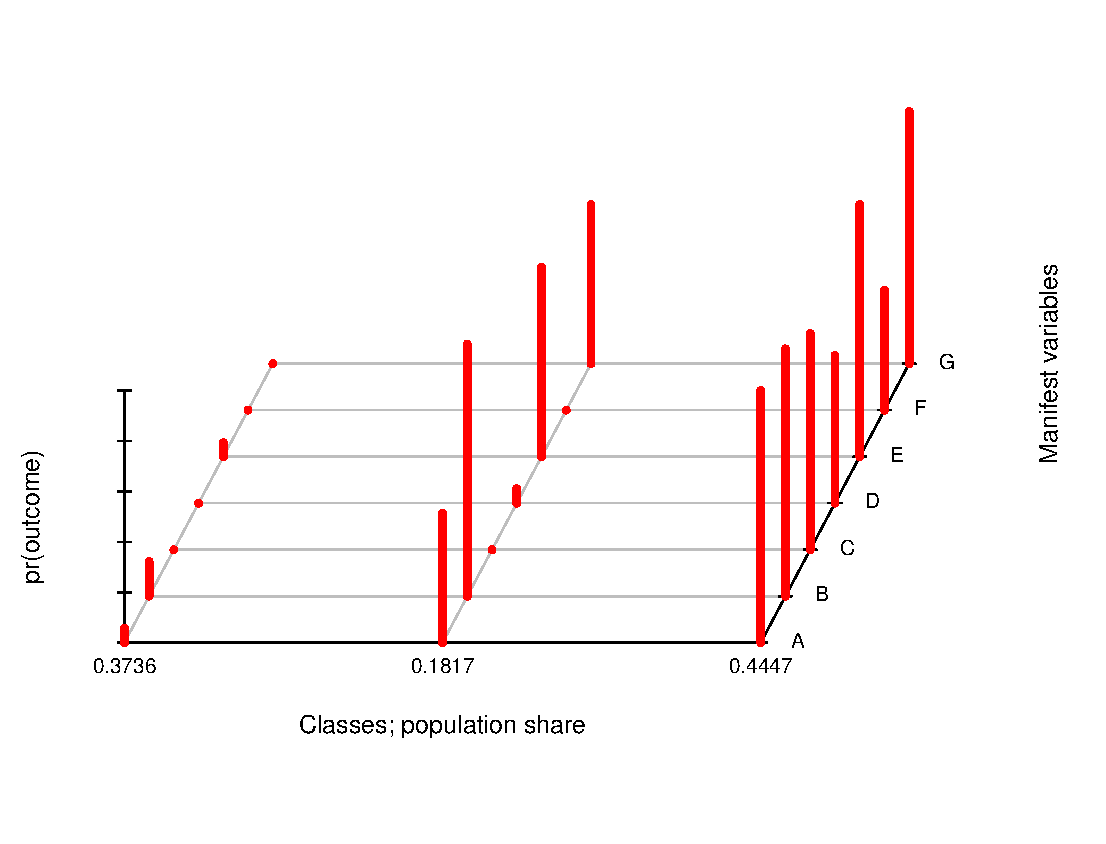
\includegraphics[scale=0.55]{carcinoma-ex.pdf}
\vspace{-0.3in}\caption{Estimation of the three-class basic latent class model using the \texttt{carcinoma} data; obtained by setting \texttt{graphs=TRUE} in the \texttt{poLCA} function call. Each group of red bars represents the conditional probabilities, by latent class, of being rated positively by each of the seven pathologists (labeled A through G). Taller bars correspond to conditional probabilities closer to 1 of a positive rating.}
\label{f.carcinoma}
\end{figure}

Figure~\ref{f.carcinoma} shows a screen capture of the estimation of model \texttt{lc3} with the \texttt{graphs} argument set to \texttt{TRUE}. As Agresti describes, the three estimated latent classes clearly correspond to a pair of classes that are consistently rated negative (37\%) or positive (44\%), plus a third ``problematic'' class representing 18\% of the population. In that class, pathologists B, E, and G tend to diagnose positive; C, D, and F tend to diagnose negative; and A is about 50/50.

The full output from model \texttt{lc3} is given below.  First, the estimated class-conditional response probabilities $\hat \pi_{jrk}$ are reported for pathologists A through G, with each row corresponding to a latent class, and each column corresponding to a diagnosis; negative in the first column, and positive in the second.  Since the manifest variables were entered as integers, the columns show the probabilities of observing a response of 1 (negative) or 2 (positive) from each pathologist, conditional on a slide being assigned to latent classes 1 through 3. Thus, for example, a slide belonging to the first (``negative'') class has a 94\% chance of being rated free from carcinoma by rater A, an 86\% chance of the same from rater B, an 100\% chance from rater C, and so forth.

Next, the output provides the estimated mixing proportions $\hat p_r$ corresponding to the share of observations belonging to each latent class.  These are the same values that appear in Figure~\ref{f.carcinoma}.  An alternative method for determining the size of the latent classes is to assign each observation to a latent class on an individual basis according to its modal posterior class membership probability.  Values using this technique are reported directly below the estimated mixing proportions.  Congruence between these two sets of population shares often indicates a good fit of the model to the data.

The next set of results simply reports the number of observations, the number of fully observed cases (for data sets with missing values and \texttt{na.rm=FALSE}), the number of estimated parameters, residual degrees of freedom, and maximum log-likelihood.  It is always worth checking to ensure that the number of residual degrees of freedom is non-negative; \texttt{poLCA} will output a warning message if this is the case.

Finally, \texttt{poLCA} outputs a number of goodness of fit statistics as described in Section~\ref{s.model-selection}.  For the \texttt{carcinoma} data, the minimum AIC and BIC criteria both indicate that the three-class model is most parsimonious: with two classes, the AIC is 664.5 and the BIC is 706.1; with three classes, the AIC decreases to 633.4 and the BIC decreases to 697.1; and with four classes, the AIC increases again to 641.6 and the BIC increases to 727.5.

\begin{verbatim}
 Conditional item response (column) probabilities,
  by outcome variable, for each class (row)

 $A
            Pr(1)  Pr(2)
 class 1:  0.9427 0.0573
 class 2:  0.4872 0.5128
 class 3:  0.0000 1.0000

 $B
            Pr(1)  Pr(2)
 class 1:  0.8621 0.1379
 class 2:  0.0000 1.0000
 class 3:  0.0191 0.9809

 $C
            Pr(1)  Pr(2)
 class 1:  1.0000 0.0000
 class 2:  1.0000 0.0000
 class 3:  0.1425 0.8575

 $D
            Pr(1)  Pr(2)
 class 1:  1.0000 0.0000
 class 2:  0.9424 0.0576
 class 3:  0.4138 0.5862

 $E
            Pr(1)  Pr(2)
 class 1:  0.9449 0.0551
 class 2:  0.2494 0.7506
 class 3:  0.0000 1.0000


 $F
            Pr(1)  Pr(2)
 class 1:  1.0000 0.0000
 class 2:  1.0000 0.0000
 class 3:  0.5236 0.4764

 $G
            Pr(1)  Pr(2)
 class 1:  1.0000 0.0000
 class 2:  0.3693 0.6307
 class 3:  0.0000 1.0000

 Estimated class population shares
  0.3736 0.1817 0.4447

 Predicted class memberships (by modal posterior prob.)
  0.3729 0.1949 0.4322

 =========================================================
 Fit for 3 latent classes:
 =========================================================
 number of observations: 118
 number of estimated parameters: 23
 residual degrees of freedom: 95
 maximum log-likelihood: -293.705

 AIC(3): 633.41
 BIC(3): 697.1357
 G^2(3): 15.26171 (Likelihood ratio/deviance statistic)
 X^2(3): 20.50336 (Chi-square goodness of fit)
\end{verbatim}


\subsection[Latent class regression modeling]{Latent class regression modeling with the \texttt{election} data}

In the \texttt{election} data set, respondents to the 2000 American National Election Study public opinion poll were asked to evaluate how well a series of traits---moral, caring, knowledgable, good leader, dishonest, and intelligent---described presidential candidates Al Gore and George~W. Bush.  Each question had four possible choices: (1)~extremely well; (2)~quite well; (3)~not too well; and (4)~not well at all.

\subsubsection{Models with one covariate}

A reasonable theoretical approach might suppose that there are three latent classes of survey respondents: Gore supporters, Bush supporters, and those who are more or less neutral. Gore supporters will tend to respond favorably towards Gore and unfavorably towards Bush, with the reverse being the case for Bush supporters.  Those in the neutral group will not have strong opinions about either candidate. We might further expect that falling into one of these three groups is a function of each individual's party identification, with committed Democrats more likely to favor Gore, committed Republicans more likely to favor Bush, and less intense partisans tending to be indifferent. We can investigate this hypothesis using a latent class regression model.

Begin by loading the \texttt{election} data into memory, and specifying a model with~12 manifest variables and \texttt{PARTY} as the lone concomitant variable.  The \texttt{PARTY} variable is coded across seven categories, from strong Democrat at~1 to strong Republican at~7.  People who primarily consider themselves Independents are at~3-4-5 on the scale.  Next, estimate the latent class regression model and assign those results to object \texttt{nes.party}.  A call to the \texttt{poLCA.reorder} command, with a subsequent re-estimation of the model, ensures that the three latent classes are assigned the same category labels in each run.
\begin{verbatim}
 > data(election)
 > f.party <- cbind(MORALG,CARESG,KNOWG,LEADG,DISHONG,INTELG,
                    MORALB,CARESB,KNOWB,LEADB,DISHONB,INTELB)~PARTY
 > nes.party <- poLCA(f.party,election,nclass=3,verbose=F)
 > probs.start <- poLCA.reorder(nes.party$probs.start,
                                order(nes.party$P,decreasing=T))
 > nes.party <- poLCA(f.party,election,nclass=3,probs.start=probs.start)
\end{verbatim}
Since the manifest variables are entered as factors, the factor labels now appear in the output of the estimated class-conditional response probabilities.  Examining these probabilities, we can confirm that the model has found the three groups separating as expected, with 27\% in the favor-Gore group, 34\% in the favor-Bush group, and 39\% in the neutral group.

This example also illustrates a shortcoming of the $\chi^2$ goodness of fit statistic, which is calculated to be over 34.5 billion.  With only 1300 observations but nearly 17 million cells in the observed cross-classification table (that is, four responses to each of 12 questions, or $4^{12}$ cells), the vast majority of the cells will contain zero cases.  For models such as this, using the $\chi^2$ statistic to assess model fit is not advised.

In addition to the information outputted for the basic model, the \texttt{poLCA} output now also includes the estimated coefficients $\boldsymbol{\hat \beta}_r$ on the covariates, and their standard errors.

\begin{figure}
\centering 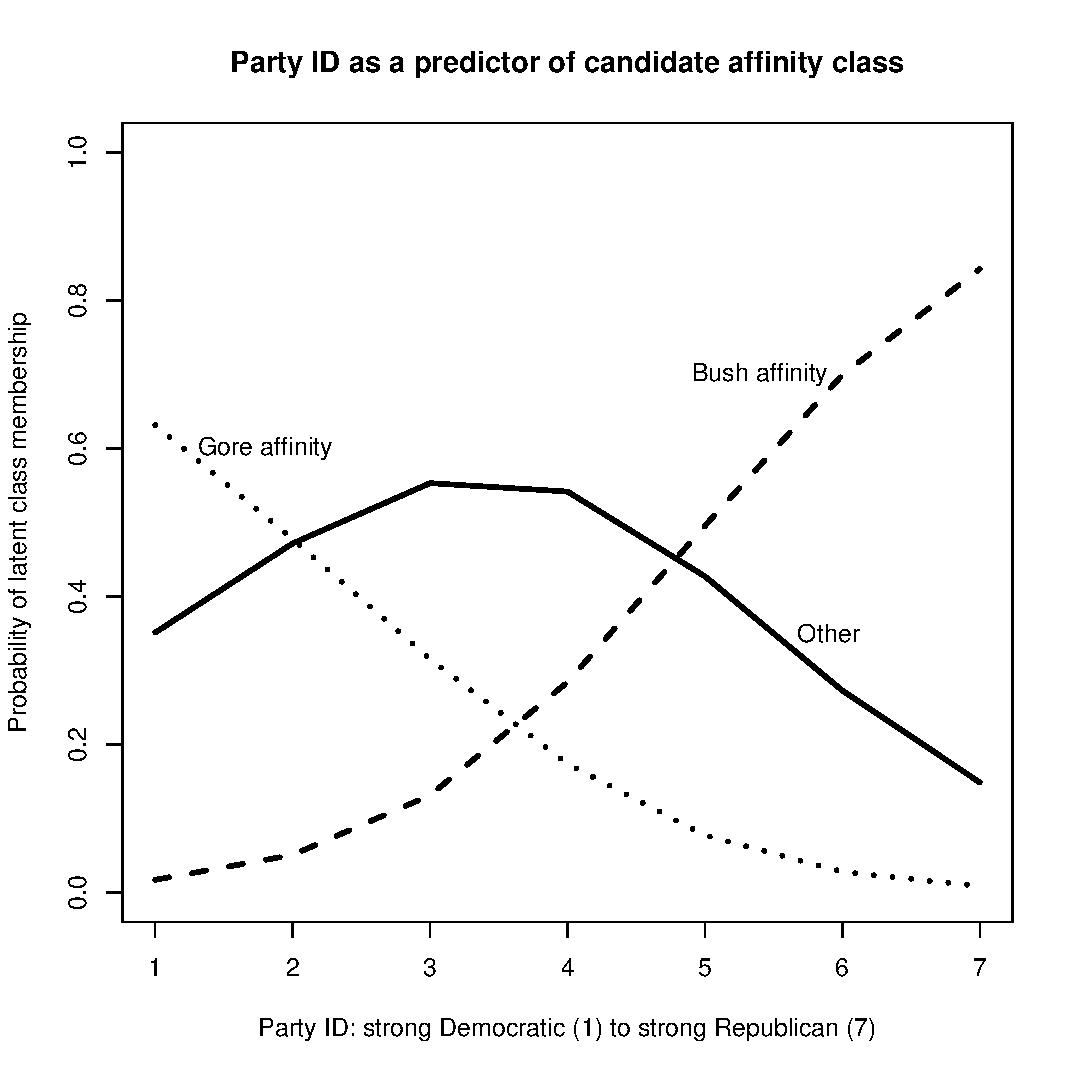
\includegraphics[scale=0.5]{election.pdf}
\caption{Predicted prior probabilities of latent class membership at varying levels of partisan self-identification. Results are from a three-class latent class regression model.}
\label{f.election}
\end{figure}

\begin{verbatim}
 =========================================================
 Fit for 3 latent classes:
 =========================================================
 2 / 1
             Coefficient  Std. error  t value  Pr(>|t|)
 (Intercept)    -3.81813     0.31109  -12.274         0
 PARTY           0.79327     0.06232   12.728         0
 =========================================================
 3 / 1
             Coefficient  Std. error  t value  Pr(>|t|)
 (Intercept)     1.16155     0.17989    6.457         0
 PARTY          -0.57436     0.06401   -8.973         0
 =========================================================
\end{verbatim}

Here, the neutral group is the first latent class, the favor-Bush group is the second latent class, and the favor-Gore group is the third latent class. Following the terminology in Section~\ref{s.terminology_r}, the log-ratio prior probability that a respondent will belong to the favor-Bush group with respect to the neutral group is $ \ln( p_{2i} / p_{1i} ) = -3.82 + 0.79 \times \texttt{PARTY}$.  Likewise, the log-ratio prior probability that a respondent will belong to the favor-Gore group with respect to the neutral group is $ \ln( p_{3i} / p_{1i} ) =  1.16 - 0.57 \times \texttt{PARTY}$.  Eq.~\ref{eq.mlogit} provides the formula for converting these log-ratios into predicted prior probabilities for each latent class.

To interpret the estimated generalized logit coefficients, we calculate and plot predicted values of $p_{ri}$, the prior probability of class membership, at varying levels of party ID. The \textsf{R} commands to do this are as follows, producing the graph in Figure~\ref{f.election}.

\begin{verbatim}
 > pidmat <- cbind(1,c(1:7))
 > exb <- exp(pidmat %*% nes.party$coeff)
 > matplot(c(1:7),(cbind(1,exb)/(1+rowSums(exb))),
           main="Party ID as a predictor of candidate affinity class",
           xlab="Party ID: strong Democratic (1) to strong Republican (7)",
           ylab="Probability of latent class membership",
           ylim=c(0,1),type="l",lwd=3,col=1)
 > text(5.9,0.35,"Other")
 > text(5.4,0.7,"Bush affinity")
 > text(1.8,0.6,"Gore affinity")
\end{verbatim}

Strong Democrats have over a 60\% prior probability of belonging to the Gore affinity group, while strong Republicans have over an 80\% prior probability of belonging to the Bush affinity group.  The prior probability of belonging to the indifferent category, labeled ``Other'', is greatest for self-identified Independents~(4) and Independents who lean Democratic~(3).

\subsubsection{Models with more than one covariate}

It is straightforward to similarly investigate models with more than one covariate.  Suppose we are interested in whether the effect of age modifies the effect of partisanship on candidate affinity.  We specify the interaction model with three covariates:
\begin{verbatim}
 > f.3cov <- cbind(MORALG,CARESG,KNOWG,LEADG,DISHONG,INTELG,
                   MORALB,CARESB,KNOWB,LEADB,DISHONB,INTELB)~PARTY*AGE
 > nes.3cov <- poLCA(f.3cov,election,nclass=3,verbose=F)

 > probs.start <- poLCA.reorder(nes.3cov$probs.start,
                                order(nes.3cov$P,decreasing=T))
 > nes.3cov <- poLCA(f.3cov,election,nclass=3,probs.start=probs.start)
\end{verbatim}
This produces the following coefficient estimates, again with the neutral group as the first latent class, the favor-Bush group as the second latent class, and the favor-Gore group as the third latent class.

\begin{verbatim}
 =========================================================
 Fit for 3 latent classes:
 =========================================================
 2 / 1
             Coefficient  Std. error  t value  Pr(>|t|)
 (Intercept)    -4.39452     0.85423   -5.144     0.000
 PARTY           0.80682     0.17614    4.581     0.000
 AGE             0.01314     0.01772    0.741     0.459
 PARTY:AGE      -0.00020     0.00363   -0.054     0.957
 =========================================================
 3 / 1
             Coefficient  Std. error  t value  Pr(>|t|)
 (Intercept)    -0.31445     0.56324   -0.558     0.577
 PARTY          -0.39923     0.19990   -1.997     0.046
 AGE             0.02967     0.01121    2.648     0.008
 PARTY:AGE      -0.00310     0.00398   -0.778     0.437
 =========================================================
\end{verbatim}

To see the effects of age on the candidate affinity of strong partisans, we first specify a matrix of hypothetical values of the covariates: \texttt{strdems} for Democrats and \texttt{strreps} for Republicans.  We then calculate and plot the predicted prior probabilities of latent class membership corresponding to each of these chosen hypothetical values (Figure~\ref{f.election2}).

\begin{figure}
\centering 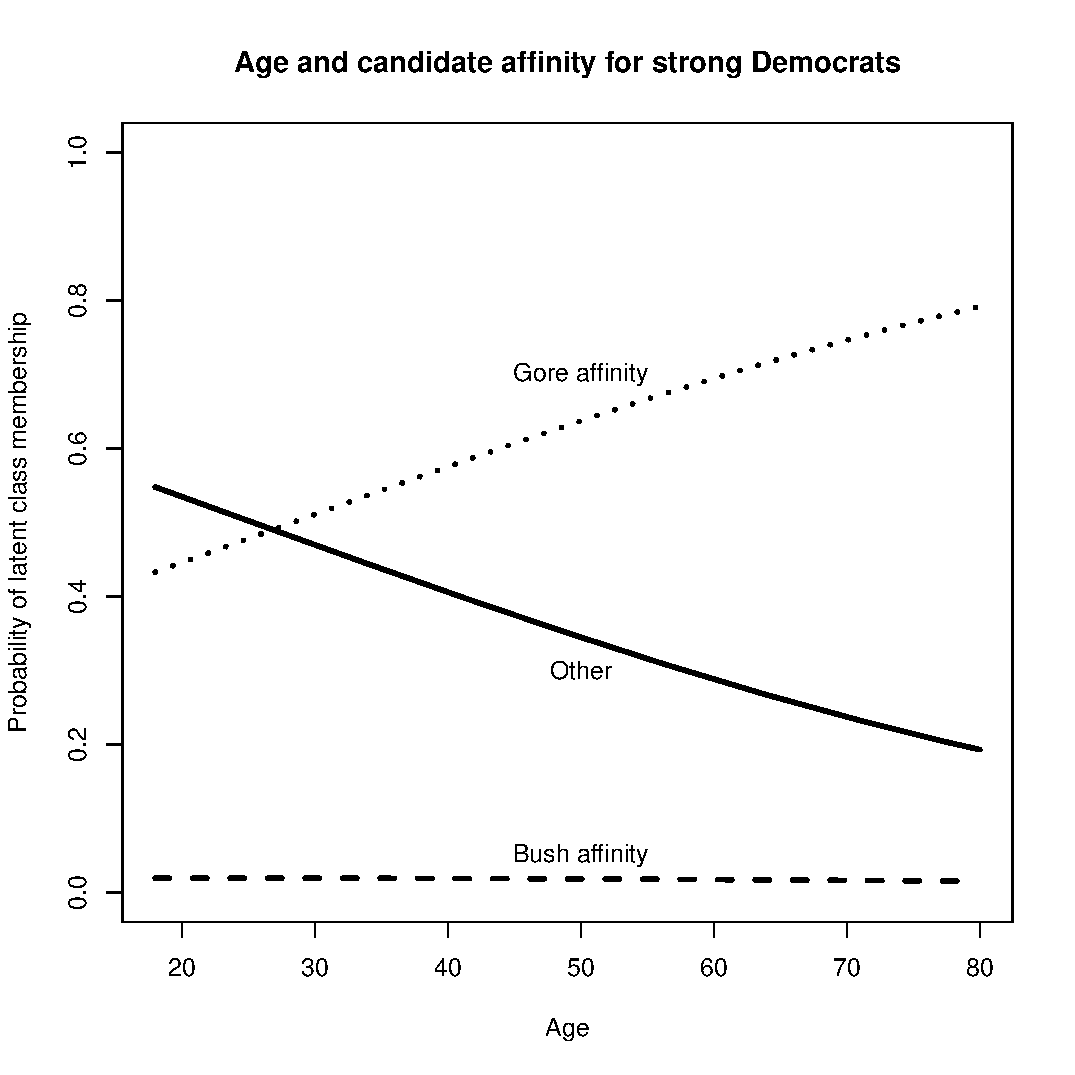
\includegraphics[scale=0.4]{election-strdems.pdf} 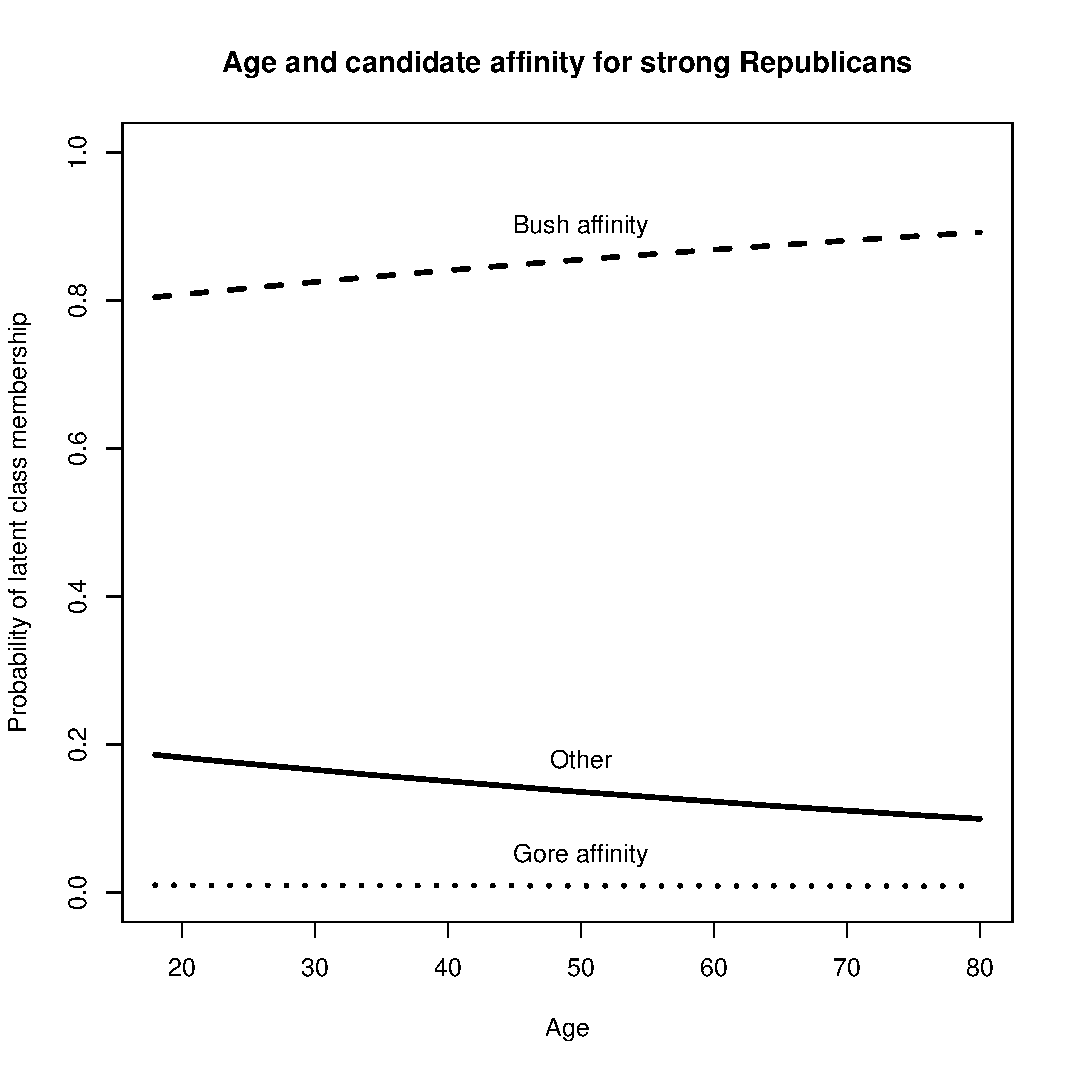
\includegraphics[scale=0.4]{election-strreps.pdf}
\caption{Predicted prior probabilities of latent class membership for strong Democrats (left) and strong Republicans (right) at ages 18-80.}
\label{f.election2}
\end{figure}

\newpage
\begin{verbatim}
 > strdems <- cbind(1,1,c(18:80),(c(18:80)*1))
 > exb.strdems <- exp(strdems %*% nes.3cov$coeff)
 > matplot(c(18:80),(cbind(1,exb.strdems)/(1+rowSums(exb.strdems))),
                  main="Age and candidate affinity for strong Democrats",
                  xlab="Age",ylab="Probability of latent class membership",
                  ylim=c(0,1),type="l",col=1,lwd=3)
\end{verbatim}

\begin{verbatim}
 > strreps <- cbind(1,7,c(18:80),(c(18:80)*7))
 > exb.strreps <- exp(strreps %*% nes.3cov$coeff)
 > matplot(c(18:80),(cbind(1,exb.strreps)/(1+rowSums(exb.strreps))),
                  main="Age and candidate affinity for strong Republicans",
                  xlab="Age",ylab="Probability of latent class membership",
                  ylim=c(0,1),type="l",col=1,lwd=3)
\end{verbatim}

As expected, regardless of age, strong Democrats are very unlikely to belong to the Bush-affinity group, and strong Republicans are very unlikely to belong to the Gore-affinity group.  However, it is interesting to observe that while strong Republicans in 2000 had extremely high levels of affinity for Bush at all ages, strong Democrats below the age of 30 tended to be just as (or more) likely to belong to the neutral group as to the Gore-affinity group.


\section{License, Contact, Versioning, Development}

\textbf{poLCA} is provided free of charge, subject to version 2 of the GPL or any later version. Users of \textbf{poLCA} are requested to cite \citet{poLCA} and \citet{LinzerLewisJSS}. Please direct all inquiries, comments, and reports of bugs to \texttt{dlinzer@emory.edu}.

\subsection{Version history}

\begin{description}
    \item[1.4:] Minor improvements, including handling of missing values and manifest variables entered as factors. Project website moved to \texttt{https://github.com/dlinzer/poLCA}. (February 21, 2013)
    \item[1.3.1:] Update to include citation to publication in \emph{Journal of Statistical Software}. (May 22, 2011)
    \item[1.3:] Addition of \texttt{poLCA.predcell} function to calculate predicted cell probabilities from the latent class model.  Addition of \texttt{poLCA.posterior} function to calculate posterior probabilities of latent class membership for specified values of manifest and concomitant variables.  Addition of \texttt{poLCA.entropy} function to calculate the entropy of the fitted cross-classification table estimated by the latent class model.  Argument \texttt{graphs=TRUE} in the \texttt{poLCA} function now plots only the final parameter estimates, rather than the updates during the estimation process.  Other minor fixes. (April~4, 2011)
    \item[1.2:] Addition of \texttt{poLCA.table} function to output cell frequencies predicted by the latent class model in tabular form. More aggressive error checking on input data, to ensure that manifest variables are entered properly as integers from one to the maximum number of outcomes for each variable. (May 11, 2010)
    \item[1.1:] Adds additional user control over ordering of latent classes and printing of model results.  New functionality to automatically estimate the latent class model multiple times to locate the global maximum likelihood solution. (November~1, 2007)
    \item[1.0:] Provides standard errors for all model parameters, and covariance matrix for regression model coefficients. Allows users to specify starting values for the estimation algorithm, to aid in convergence and increase control over model output. (April~4, 2007)
    \item[0.9:] First public release. (June~1, 2006)
\end{description}

\subsection{Planned developments}

\textbf{poLCA} is still undergoing active development.  Planned extensions include:

\begin{itemize}
    \item Incorporation of sampling weights.
    \item Flexibility to relax the assumption of local independence among selected manifest variables.
    \item Accommodation of user-specified constraints on selected parameters $\pi_{jrk}$, as a way to simplify models, achieve model identifiability, test substantive hypotheses, and analyze model fit. Such constraints might, for example, require selected response probabilities to be set equal to one another across different classes, across manifest variables within classes, or equal to fixed constant values, as in \citet{Goodman1974}.  This extension would also permit the estimation of so-called ``simultaneous'' latent class models across multiple groups where the groups are already known (or theorized) to exist in the data \citep{CloggGoodman1986}.
\end{itemize}

\newpage
\bibliography{poLCA-manual}

\end{document}
